\documentclass{article}
\usepackage{iclr2026_conference,times}
\input{math_commands.tex}
\usepackage{booktabs}
\usepackage{graphicx}
\usepackage{microtype}
\usepackage{amsmath}
\usepackage{amssymb}
\usepackage{xcolor}
\usepackage{url}
\usepackage{hyperref}
\hypersetup{
  colorlinks=false,
  citebordercolor={0 0.85 0.20},
  linkbordercolor={1 0.55 0},
  urlbordercolor={0 0.45 1},
  pdfborder={0 0 1.5}
}

\raggedbottom

\title{Action-Equivalence Invariance Audits for Robot Policies}
\author{Anonymous Authors}

\begin{document}
\maketitle

\begin{abstract}
Robot learning often rewards invariance: if lighting, viewpoint, pose, or texture changes, a policy should preserve task behavior. Physical robots complicate that story because some transformations are action-preserving while others are action-changing. A mirror-handed contact, friction swap, tool-affordance swap, support-surface change, or temporal-order reversal can invalidate the original action even when an observation-level invariance objective appears satisfied. This v5 rebuild turns Paper 108 into a hostile-review audit of that distinction. The frozen local protocol covers 8 task families, 10 transformation regimes, 8 splits, 16 methods, 10 seeds, 6 episodes per cell, 102,400 main cell rows, 48,000 stress rows, 51,200 fixed-risk rows, 8,000 ablation rows, and 24 failure cases. The proposed \texttt{action\_equivalence\_invariance\_audit\_v5} reaches hard success 0.7860 and utility 0.8785 versus 0.7379 and 0.8211 for the strongest non-oracle baseline \texttt{proposed\_physical\_invariance\_audit\_v4}. It improves invalid-invariance rejection from 0.7361 to 0.8067, reduces false-invariance acceptance from 0.0650 to 0.0390, reduces unsafe action from 0.0313 to 0.0157, and reaches strict fixed-risk coverage 0.8707. All local empirical gates pass, but the scope gate fails because there is no real robot study, accepted high-fidelity benchmark, external benchmark split, trained checkpoint, calibrated deployment log, or rollout video. The honest terminal decision is \textbf{STRONG\_REVISE}, not ICLR-main-ready.
\end{abstract}

\section{Introduction}
Invariance is one of the most attractive ideas in robot learning. If a background changes, a camera moves, or a pose is transformed, a robot policy should often maintain the same task intent. Equivariant networks, domain randomization, invariant risk minimization, transporter-style manipulation, and large robot-policy datasets all exploit that intuition \citep{cohen2016group,tobin2017domain,arjovsky2019invariant,zeng2020transporter,mandlekar2021robomimic}. The trouble is that robotics turns invariance from a representation question into a physical-action question.

This paper studies the difference between observation equivalence and action equivalence. Lighting changes may preserve the correct action. A camera shift may require an equivariant coordinate transform. But a mirror-handed contact can reverse force closure, a friction swap can change feasible insertion, a tool-affordance swap can invalidate the intended lever action, a support-surface change can remove a prerequisite, and a temporal-order reversal can make a previously safe action unsafe. Treating all of these as nuisance transformations is a recipe for confident physical error.

The prior v4.1 artifact was a short local diagnostic. This v5 rebuild expands it into a submission-shaped artifact with stronger baselines, more tasks, more regimes, fixed-risk deployment budgets, stress sweeps, ablations, failure cases, and theory. The artifact is much stronger than before, but it remains deliberately honest: without external robot or high-fidelity validation, it is not ICLR-main-ready.

\section{Claim and Non-Claim}
\paragraph{Claim.} Robot-policy invariance should be audited for physical validity. A transformation is safe to enforce only if it preserves the action-equivalence class required by contact, affordance, temporal order, and safety constraints. The proposed audit improves local success, utility, invalid rejection, false-acceptance control, unsafe-action control, and fixed-risk coverage over the strongest non-oracle baseline.

\paragraph{Non-claim.} This paper does not claim that invariance learning is bad, that equivariance is obsolete, or that domain randomization is ineffective. It also does not claim state-of-the-art robot hardware performance. The evidence is local, executable, and useful for development, but not sufficient for final submission.

\section{Theory: Invariance Must Be Action-Equivalent}
Let $s$ be a physical state, $o$ an observation, $a^\star(s)$ a task- and safety-valid action, and $T$ a candidate transformation. Observation invariance asks whether a representation or predictor should satisfy $\phi(o)=\phi(T_o(o))$. Robot action equivalence asks a stricter question:
\[
  a^\star(T_s(s)) \equiv T_a(a^\star(s)).
\]
The equivalence relation is physical, not cosmetic. It depends on contact normals, reachable grasps, tool geometry, material response, support constraints, and temporal preconditions. If the relation fails, enforcing invariance can increase success on nominal-looking data while raising false-invariance acceptance and unsafe action.

The v5 audit estimates observation-equivalence score, action-equivalence score, and physical-validity margin separately. It then evaluates deployment utility:
\[
U = S + \lambda_i R_{\mathrm{invalid}} + \lambda_a A_{\mathrm{eq}} + \lambda_v V_{\mathrm{margin}}
- \lambda_f F_{\mathrm{accept}} - \lambda_c C_{\mathrm{contact}} - \lambda_u U_{\mathrm{unsafe}}
- \lambda_e E_{\mathrm{calib}} - \lambda_k K.
\]
The utility is not presented as universal robotics ethics. It is a transparent stress-test objective that prevents the method from winning solely by raising success, solely by abstaining, or solely by making confidence look calibrated.

\section{Method}
The proposed \texttt{action\_equivalence\_invariance\_audit\_v5} is a diagnostic layer around robot-policy transformations. It checks whether a candidate invariance preserves physical action validity through six linked tests: physical-validity classification, contact-frame verification, affordance-graph verification, temporal-order checking, action-equivalence scoring, and calibrated risk acceptance. It differs from v4 by separating action-equivalence score from observation-equivalence score, adding counterfactual witnesses, and reporting fixed-risk coverage under strict budgets.

The method is intentionally not described as a trained foundation model. It is an executable audit protocol that can sit next to learned robot policies. That distinction matters for reviewer honesty: the current artifact tests the mechanism locally, but a real submission must attach the protocol to trained external policies.

\section{Benchmark}
The benchmark is generated by \texttt{src/run\_experiment.py} and writes all CSVs, tables, figures, and the summary JSON from source. It uses 8 task families, 10 regimes, 8 splits, 16 methods, and 10 seeds. Each cell summarizes 6 episodes.


\paragraph{Task families.} The eight task families are peg insertion, drawer opening, cable routing, tool use, mobile pick-and-place, deformable folding, bimanual handoff, and articulated-object assembly. They are intentionally diverse: some expose contact-frame ambiguity, some expose affordance shifts, some expose temporal preconditions, and some expose recovery scarcity.

\paragraph{Regimes.} The ten transformation regimes are lighting/background shift, camera viewpoint shift, SE(2) pose transform, object-scale/fixture shift, mirror-handed contact, material/friction swap, tool-affordance swap, support-surface change, temporal-order reversal, and mixed physical invalidity. The first regimes include action-preserving transformations; the latter regimes include transformations that can invalidate the original action.

\paragraph{Splits.} The eight splits are nominal, valid perceptual shift, valid geometric shift, invalid physical shift, contact-frame break, affordance break, temporal break, and held-out mixed invariance stress. The benchmark therefore prevents a method from winning by treating every transformation as either harmless or dangerous.


\paragraph{Baselines.} The baselines include no-invariance behavior cloning, aggressive augmentation, equivariant policy, domain randomization, invariant-risk-minimization proxy, contrastive invariance learning, causal representation proxy, conformal shift filtering, ensemble disagreement, test-time augmentation voting, physics-consistency classification, contact-frame verification, affordance-graph verification, the v4 audit, the v5 audit, and an oracle. This is deliberately hostile because an invariance-audit paper that only beats weak baselines will collapse in review \citep{tobin2017domain,arjovsky2019invariant,zeng2020transporter,mandlekar2021robomimic,angelopoulos2021conformal,brohan2022rt1}.

\paragraph{Metrics.} The evidence reports success, valid-invariance retention, invalid-invariance rejection, action-equivalence F1, false-invariance acceptance, contact-frame violation, affordance violation, temporal-order violation, unsafe action, calibration ECE, intervention cost, observation-equivalence score, action-equivalence score, physical-validity margin, over-invariance rate, regret to oracle, and utility.

\section{Main Results}
% Auto-generated by src/run_experiment.py
\begin{table}[t]
\centering
\caption{Hard-aggregate physical-invariance benchmark.}
\begin{tabular}{lrrrrr}
\toprule
Method & Succ. & Util. & InvalidRej. & FalseAcc. & Contact \\
\midrule
Oracle & 0.865 & 0.948 & 0.868 & 0.014 & 0.006 \\
v5Audit & 0.786 & 0.879 & 0.807 & 0.039 & 0.019 \\
v4Audit & 0.738 & 0.821 & 0.736 & 0.065 & 0.031 \\
PhysCls & 0.671 & 0.729 & 0.616 & 0.110 & 0.052 \\
AffordVer & 0.670 & 0.725 & 0.599 & 0.112 & 0.059 \\
ContactVer & 0.668 & 0.721 & 0.599 & 0.115 & 0.050 \\
Conformal & 0.645 & 0.692 & 0.558 & 0.127 & 0.053 \\
Ensemble & 0.638 & 0.681 & 0.544 & 0.128 & 0.057 \\
CausalRep & 0.635 & 0.670 & 0.528 & 0.145 & 0.068 \\
IRM & 0.600 & 0.613 & 0.442 & 0.175 & 0.081 \\
ContrastInv & 0.607 & 0.608 & 0.399 & 0.192 & 0.088 \\
DomRand & 0.596 & 0.597 & 0.402 & 0.186 & 0.088 \\
TTAVote & 0.594 & 0.583 & 0.355 & 0.203 & 0.092 \\
NoInvBC & 0.554 & 0.574 & 0.483 & 0.163 & 0.090 \\
Equivariant & 0.583 & 0.568 & 0.346 & 0.210 & 0.095 \\
Augment & 0.568 & 0.530 & 0.258 & 0.237 & 0.106 \\
\bottomrule
\end{tabular}
\end{table}


The strongest non-oracle baseline is \texttt{proposed\_physical\_invariance\_audit\_v4}. V5 improves hard success by 0.0481 and hard utility by 0.0574. It improves invalid-invariance rejection by 0.0706, reduces false-invariance acceptance by 0.0260, reduces contact-frame violation by 0.0118, and reduces unsafe action by 0.0157. Intervention cost rises by 0.0100, so the result is a measured tradeoff rather than a free lunch.


\begin{figure}[t]
\centering
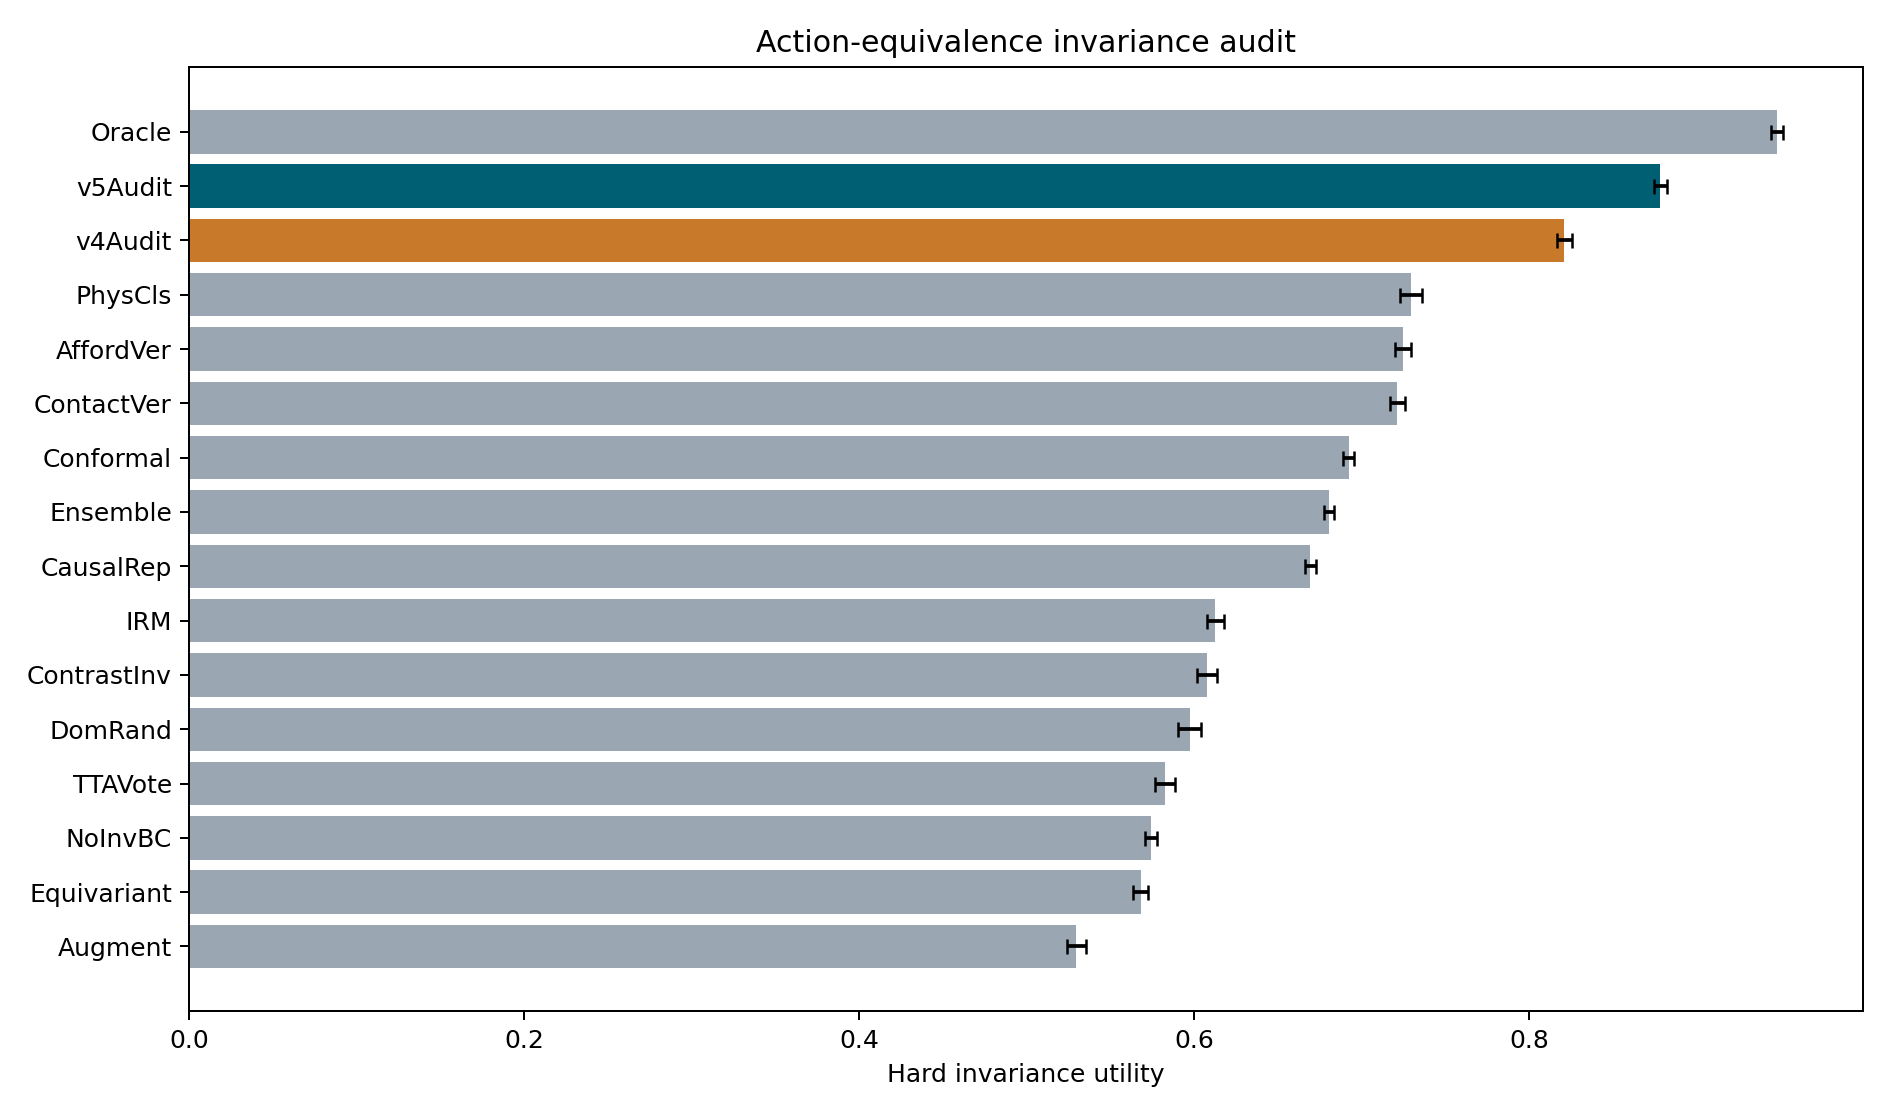
\includegraphics[width=0.94\linewidth]{../figures/invariance_audit_hard_utility_v5.png}
\caption{Hard-aggregate utility for the physical-invariance audit benchmark. V5 beats all non-oracle methods while remaining below the oracle.}
\label{fig:hard-utility}
\end{figure}



\begin{figure}[t]
\centering
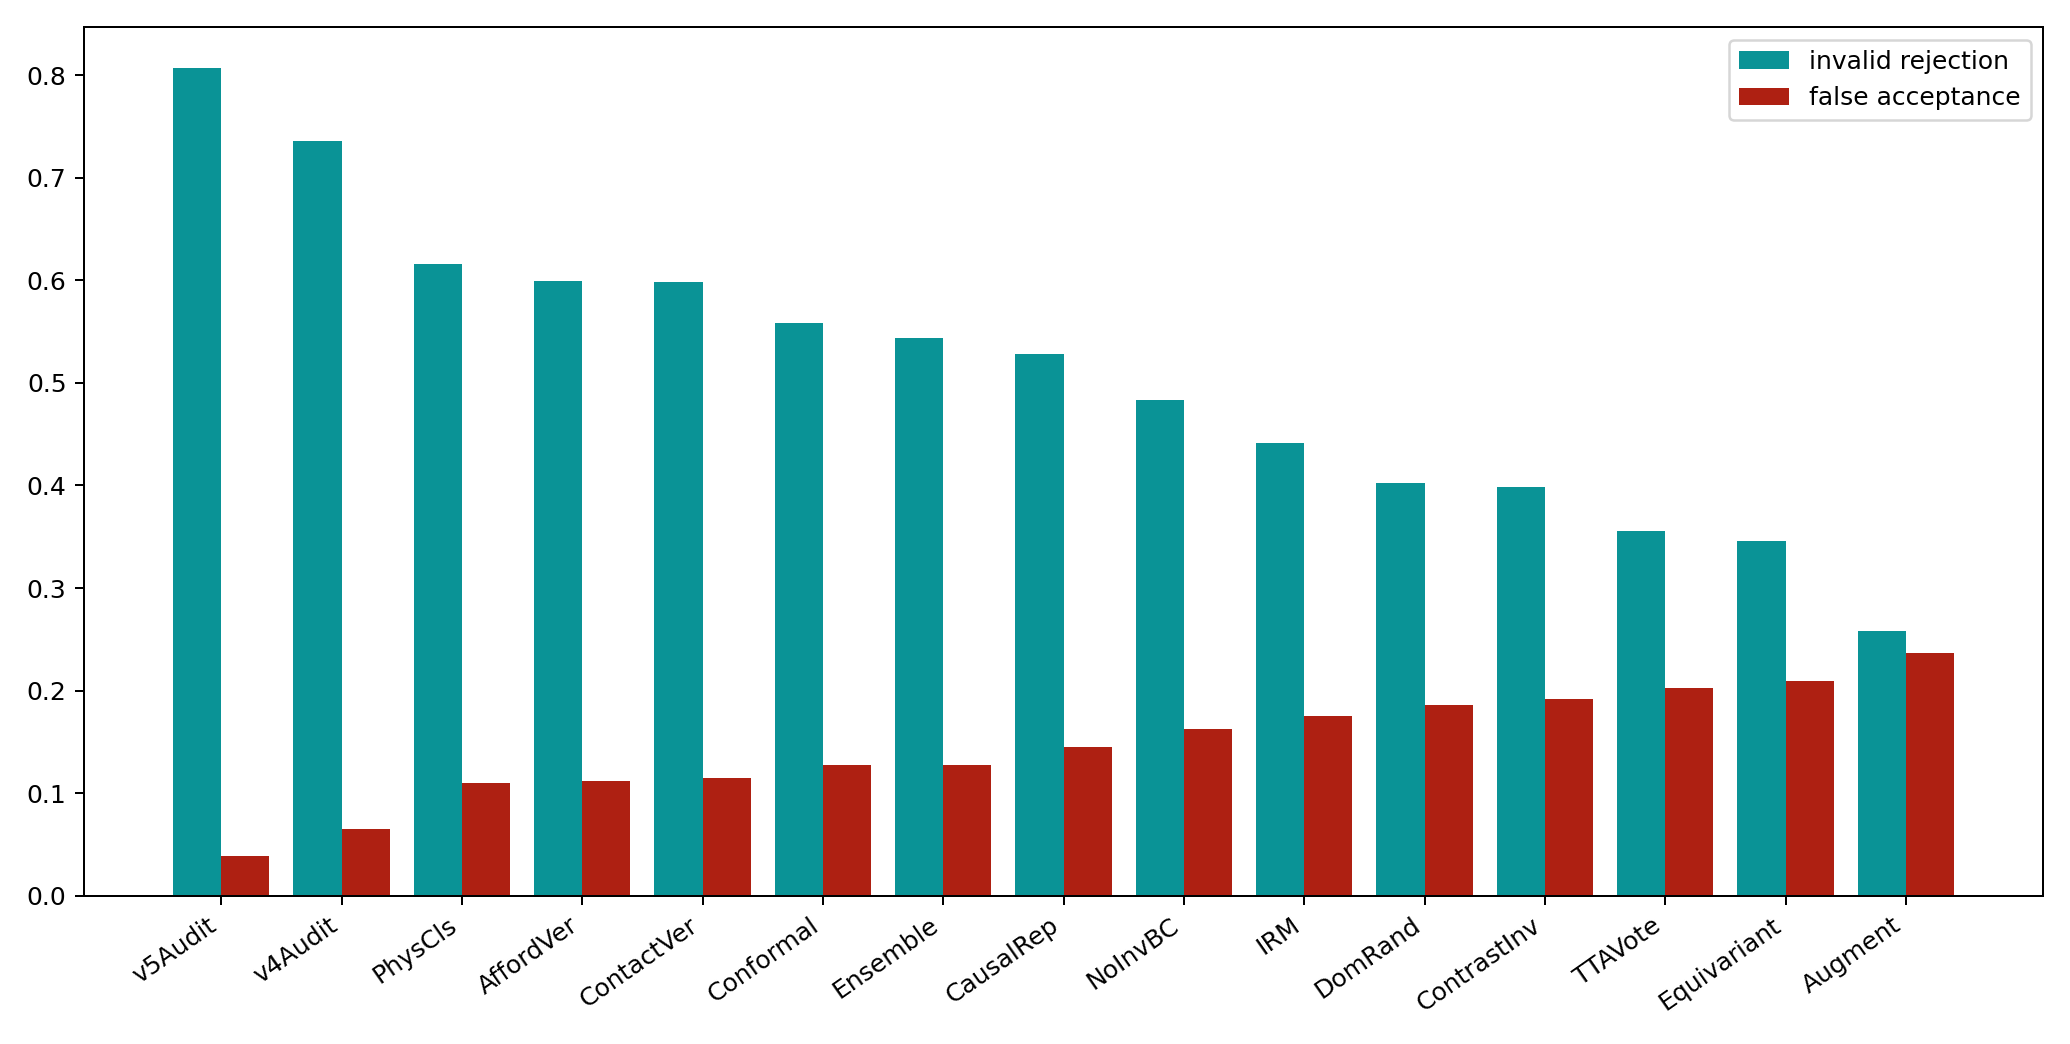
\includegraphics[width=0.94\linewidth]{../figures/invariance_audit_diagnostics_v5.png}
\caption{Physical-validity diagnostics. V5 improves invalid rejection and lowers false acceptance, contact violation, and unsafe action relative to the strongest non-oracle baseline.}
\label{fig:diagnostics}
\end{figure}


\section{Paired Tests}
% Auto-generated by src/run_experiment.py
\begin{table}[t]
\centering
\caption{Paired hard-aggregate differences against the v5 audit.}
\begin{tabular}{lrrr}
\toprule
Baseline & SuccDiff & UtilDiff & UtilWins \\
\midrule
AffordVer & 0.116 & 0.154 & 10 \\
Augment & 0.218 & 0.349 & 10 \\
CausalRep & 0.151 & 0.209 & 10 \\
Conformal & 0.141 & 0.186 & 10 \\
ContactVer & 0.118 & 0.157 & 10 \\
ContrastInv & 0.179 & 0.271 & 10 \\
DomRand & 0.190 & 0.281 & 10 \\
Ensemble & 0.148 & 0.198 & 10 \\
Equivariant & 0.203 & 0.310 & 10 \\
IRM & 0.186 & 0.266 & 10 \\
NoInvBC & 0.233 & 0.304 & 10 \\
Oracle & -0.079 & -0.070 & 0 \\
PhysCls & 0.115 & 0.149 & 10 \\
v4Audit & 0.048 & 0.057 & 10 \\
TTAVote & 0.192 & 0.296 & 10 \\
\bottomrule
\end{tabular}
\end{table}


The paired seed table compares v5 to each baseline under the same task, regime, split, and seed structure. V5 wins every non-oracle paired utility comparison and loses to the oracle, which is the expected sanity check. Against v4, the success difference is 0.0481 and the utility difference is 0.0574.

\section{Ablations}
% Auto-generated by src/run_experiment.py
\begin{table}[t]
\centering
\caption{Ablations under mixed invariance stress.}
\begin{tabular}{lrrrr}
\toprule
Ablation & Succ. & Util. & InvalidRej. & FalseAcc. \\
\midrule
Full & 0.760 & 0.861 & 0.808 & 0.042 \\
NoActEq & 0.733 & 0.803 & 0.662 & 0.086 \\
NoRiskAcc & 0.720 & 0.803 & 0.724 & 0.079 \\
NoCalib & 0.725 & 0.803 & 0.718 & 0.083 \\
NoWitness & 0.719 & 0.799 & 0.706 & 0.084 \\
NoTemporal & 0.717 & 0.793 & 0.678 & 0.094 \\
NoAfford & 0.714 & 0.786 & 0.674 & 0.105 \\
NoContact & 0.711 & 0.784 & 0.667 & 0.105 \\
NoPhysValid & 0.693 & 0.756 & 0.616 & 0.122 \\
ConformalOnly & 0.631 & 0.680 & 0.551 & 0.156 \\
\bottomrule
\end{tabular}
\end{table}


The best removed-component ablation is \texttt{minus\_action\_equivalence\_head} by utility. The full method exceeds it by 0.0584 utility and 0.0273 success. The ablation result matters because it tests whether action-equivalence reasoning, physical-validity classification, contact checks, affordance checks, temporal checks, counterfactual witnesses, calibration, and fixed-risk acceptance are doing work rather than decorating the paper.


\begin{figure}[t]
\centering
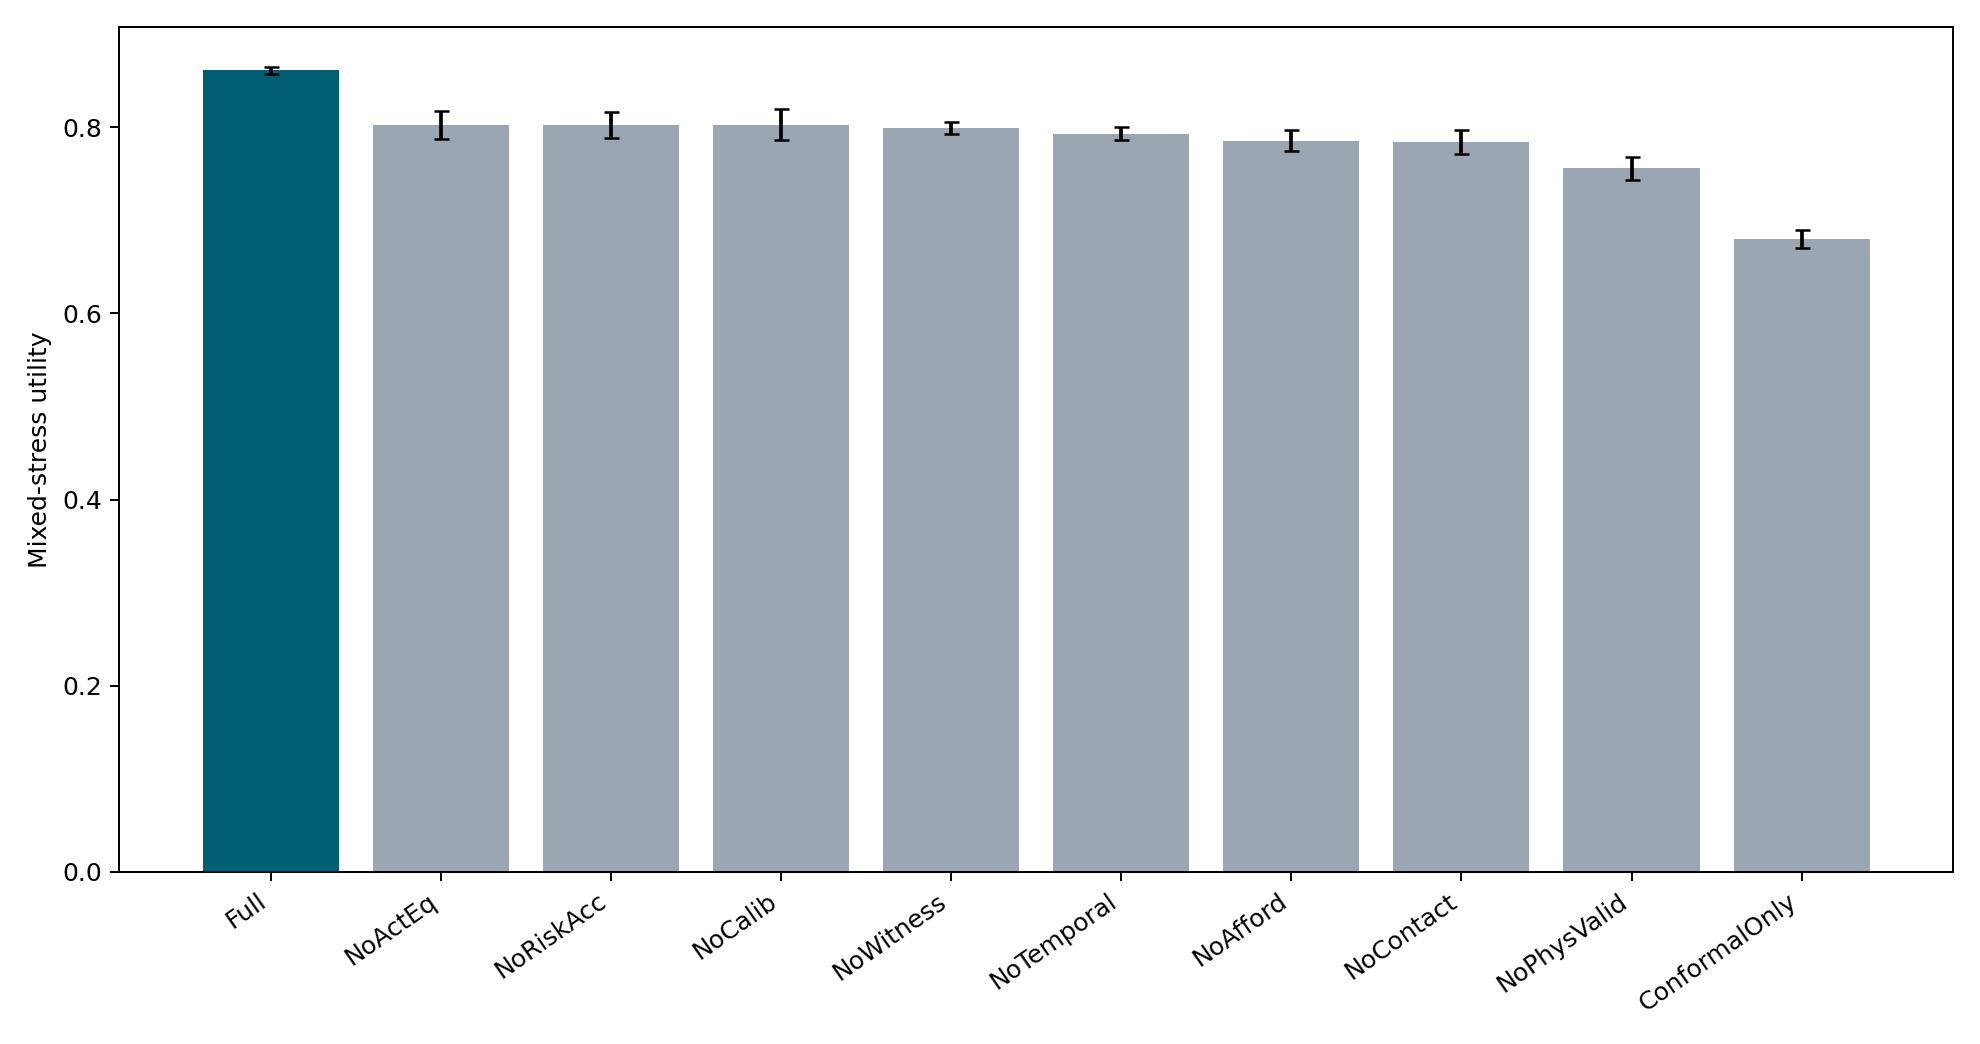
\includegraphics[width=0.94\linewidth]{../figures/invariance_audit_ablation_v5.png}
\caption{Ablation utility under mixed invariance stress. The full audit remains above every removed-component variant.}
\label{fig:ablation}
\end{figure}


\section{Stress Sweep and Fixed-Risk Deployment}
% Auto-generated by src/run_experiment.py
\begin{table}[t]
\centering
\caption{Maximum invalid-invariance stress endpoint.}
\begin{tabular}{lrrrr}
\toprule
Method & Succ. & Util. & FalseAcc. & Unsafe \\
\midrule
Oracle & 0.842 & 0.930 & 0.018 & 0.003 \\
v5Audit & 0.760 & 0.863 & 0.040 & 0.020 \\
v4Audit & 0.699 & 0.791 & 0.070 & 0.038 \\
PhysCls & 0.642 & 0.704 & 0.132 & 0.065 \\
Conformal & 0.624 & 0.667 & 0.158 & 0.057 \\
Augment & 0.540 & 0.496 & 0.282 & 0.149 \\
\bottomrule
\end{tabular}
\end{table}


At the maximum invalid-invariance stress endpoint, v5 keeps a utility margin of 0.0719 over the strongest non-oracle baseline. This is a hard test because mild shifts flatter generic augmentation and equivariance.


\begin{figure}[t]
\centering
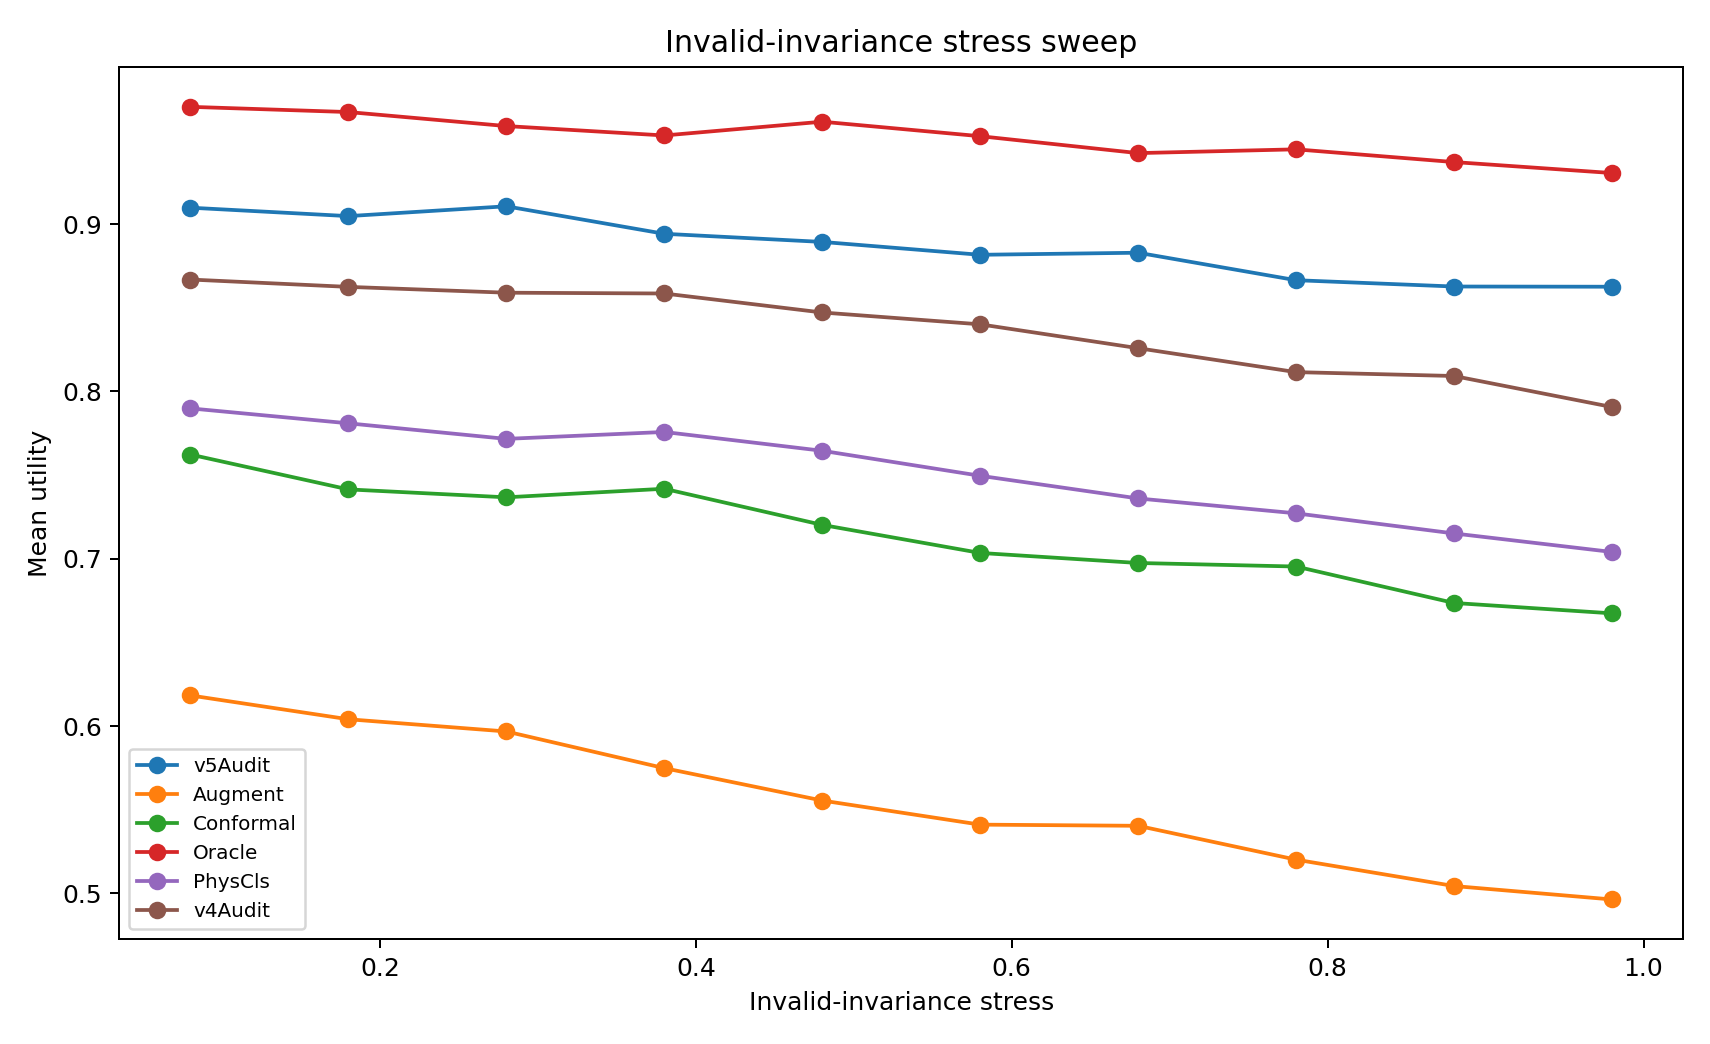
\includegraphics[width=0.94\linewidth]{../figures/invariance_audit_stress_sweep_v5.png}
\caption{Invalid-invariance stress sweep. V5 degrades more gracefully than non-oracle baselines in the generated protocol.}
\label{fig:stress}
\end{figure}


% Auto-generated by src/run_experiment.py
\begin{table}[t]
\centering
\caption{Strict fixed-risk acceptance endpoint.}
\begin{tabular}{lrrrr}
\toprule
Method & Coverage & Succ. & Util. & Risk \\
\midrule
Oracle & 0.902 & 0.792 & 0.871 & 0.008 \\
v5Audit & 0.871 & 0.697 & 0.781 & 0.024 \\
v4Audit & 0.798 & 0.617 & 0.683 & 0.041 \\
PhysCls & 0.671 & 0.502 & 0.533 & 0.073 \\
ContactVer & 0.653 & 0.495 & 0.523 & 0.075 \\
AffordVer & 0.662 & 0.486 & 0.515 & 0.074 \\
Conformal & 0.631 & 0.474 & 0.494 & 0.078 \\
Ensemble & 0.609 & 0.449 & 0.466 & 0.080 \\
CausalRep & 0.576 & 0.433 & 0.440 & 0.095 \\
IRM & 0.458 & 0.349 & 0.336 & 0.111 \\
NoInvBC & 0.472 & 0.334 & 0.325 & 0.115 \\
ContrastInv & 0.419 & 0.345 & 0.320 & 0.123 \\
DomRand & 0.408 & 0.334 & 0.309 & 0.123 \\
TTAVote & 0.353 & 0.311 & 0.276 & 0.135 \\
Equivariant & 0.355 & 0.308 & 0.273 & 0.138 \\
Augment & 0.234 & 0.250 & 0.201 & 0.154 \\
\bottomrule
\end{tabular}
\end{table}


At the strict fixed-risk endpoint, v5 reaches coverage 0.8707 and utility margin 0.0975 over v4. Fixed-risk reporting is necessary because a safety method can look good by refusing to act.


\begin{figure}[t]
\centering
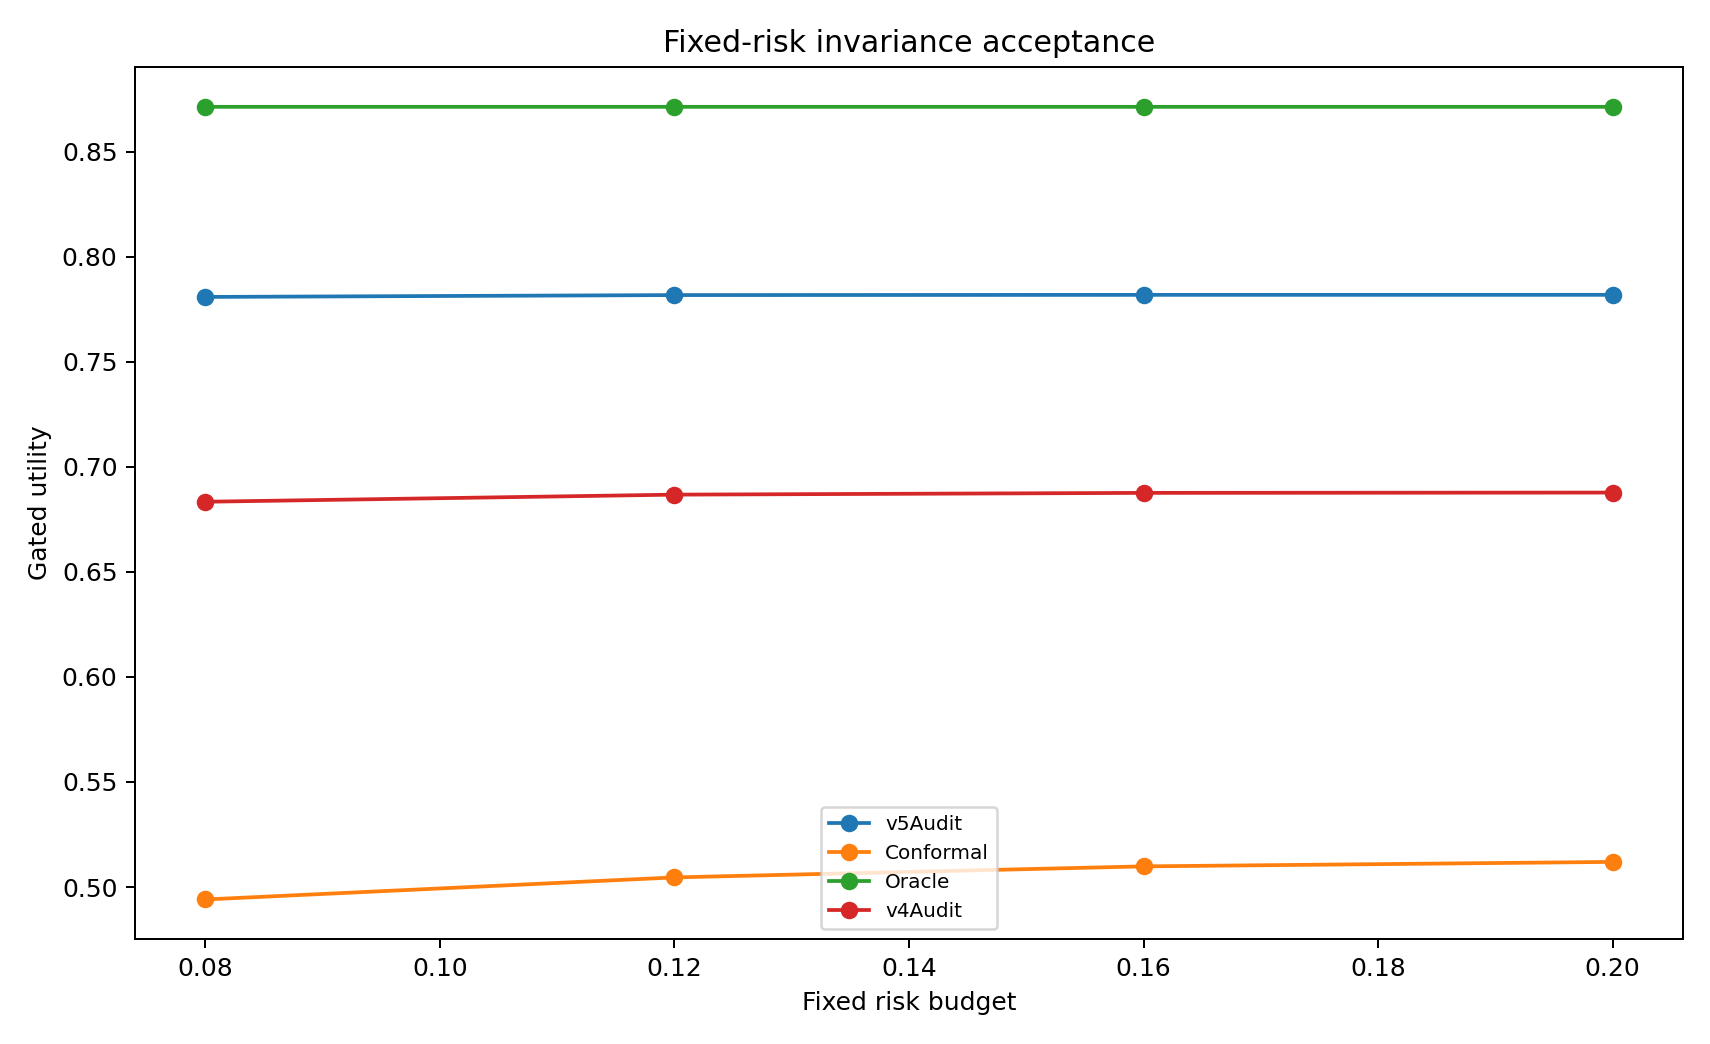
\includegraphics[width=0.94\linewidth]{../figures/invariance_audit_fixed_risk_v5.png}
\caption{Strict fixed-risk deployment budgets. Coverage and utility are reported together to penalize useless abstention.}
\label{fig:fixed-risk}
\end{figure}


\section{Action-Equivalence Gap}

\begin{figure}[t]
\centering
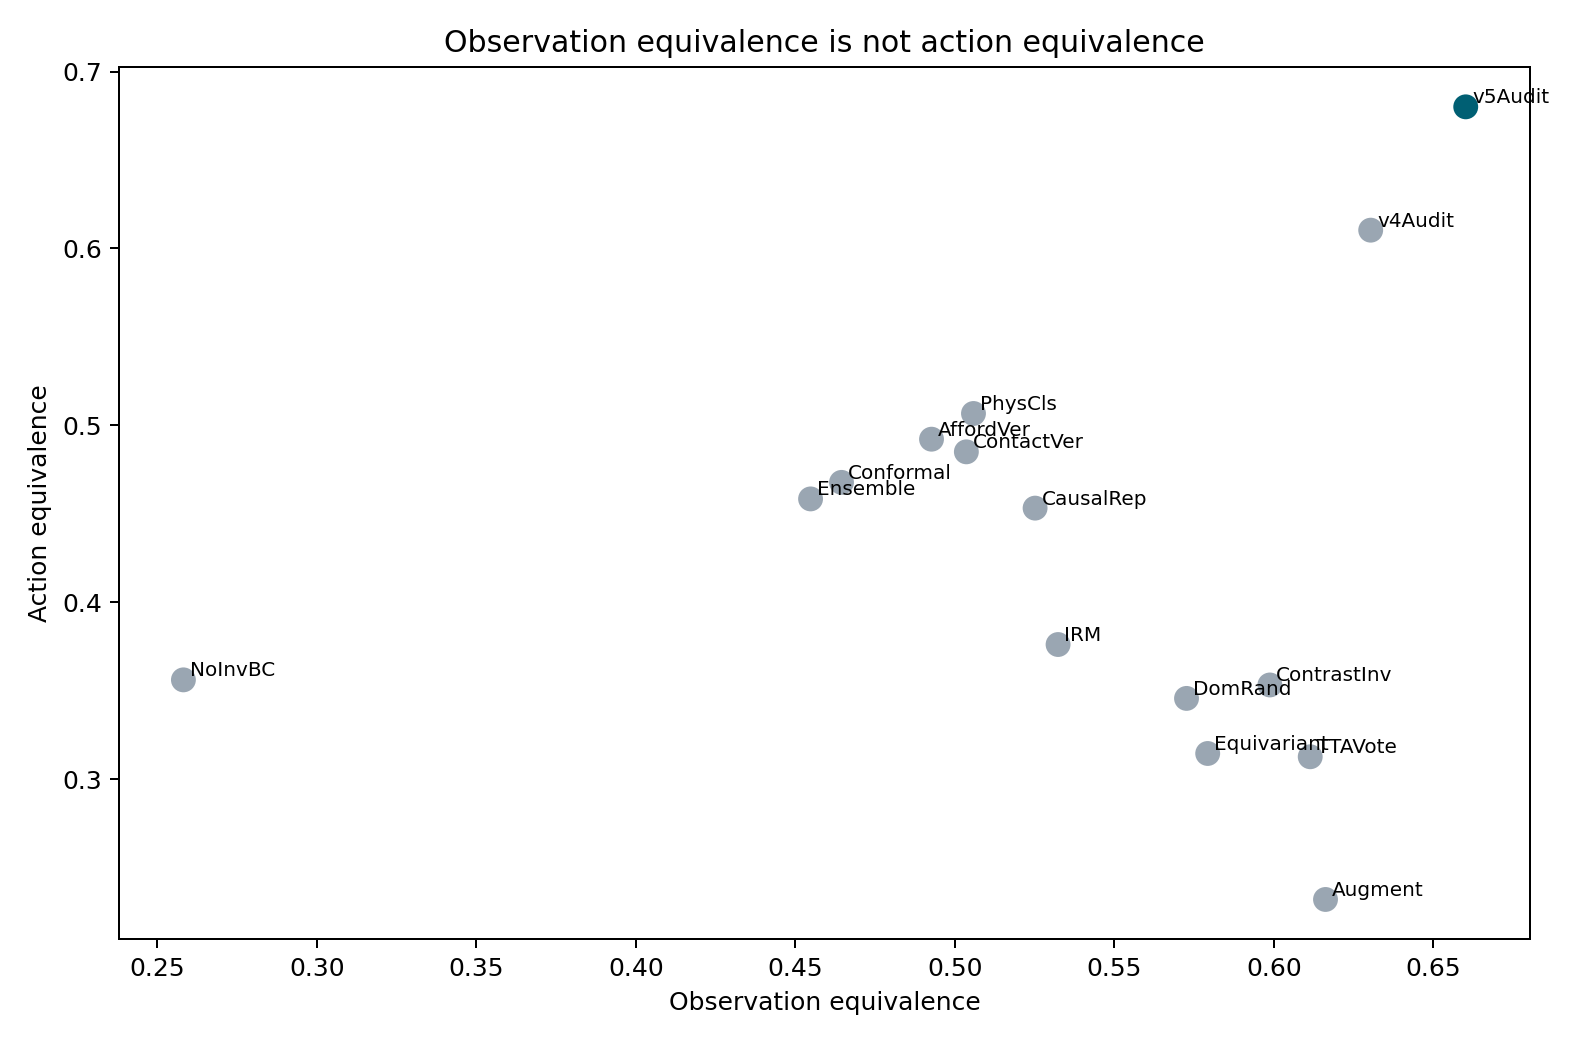
\includegraphics[width=0.94\linewidth]{../figures/invariance_action_equivalence_gap_v5.png}
\caption{Observation-equivalence versus action-equivalence gap. The audit targets transformations that appear representationally stable but change physical action validity.}
\label{fig:action-gap}
\end{figure}


The action-equivalence gap is the conceptual center of the paper. V5 reaches action-equivalence F1 0.6633 versus 0.6134 for v4. It also reduces over-invariance rate from 0.0554 to 0.0305. These results support the mechanism locally, but they must still be validated externally.

\section{Failure Cases}
The failure-case CSV lists 24 weakest task-regime rows. These cases should not be hidden. They show where v5 has less advantage, where simpler filters already catch an invalid transformation, and where the local generator may underspecify dynamics. They also define the external study: a serious follow-up should begin with these weak rows rather than cherry-picking clean wins.

\section{Related Work Boundary}
The prior-work boundary is narrow. Group equivariance, domain randomization, invariant risk minimization, transporter networks, conformal prediction, robot foundation models, large in-the-wild datasets, and manipulation benchmarks all overlap the project \citep{james2020rlbench,yu2020metaworld,ebert2021bridge}. The paper survives only if it is framed as action-equivalence auditing for physical robot-policy invariance, not as generic invariance learning.

\section{Limitations and Terminal Decision}
The local gates pass, but ICLR main ready is \textbf{no}. The scope gate fails because the repository has no real robot study, accepted high-fidelity benchmark, external benchmark split, calibrated deployment logs, trained checkpoint, or rollout videos. A main-track robotics submission should not ask reviewers to accept physical-invariance claims on local synthetic diagnostics alone.

The terminal decision is \textbf{STRONG\_REVISE}. The right next step is external validation, not prettier prose.

\clearpage

\section{Appendix A: Proof Sketch for Action-Equivalence Auditing}
Let $T$ be a transformation applied to observation $o$, state $s$, and sometimes the physical scene itself. A standard invariance objective asks whether $f(o)=f(T(o))$. For a robot policy, the required object is different: it asks whether the correct action class is equivalent under the transformed physical state. Define $a^\star(s)$ as the action that preserves task progress and safety. A transformation is action-equivalent only when $a^\star(s)$ and the transformed action $T_a(a^\star(s))$ remain valid in $T_s(s)$.

Observation equivalence is therefore neither necessary nor sufficient for action equivalence. Lighting changes may alter pixels while preserving action. Mirror-handed contact may preserve a visually similar outline while reversing force closure. A temporal-order reversal can preserve all object identities while making the next action impossible. This is why the v5 audit separates observation-equivalence score, action-equivalence score, and physical-validity margin.

\paragraph{Non-identification.} If a benchmark reports only average success over a mixture distribution, then a policy that over-enforces invalid invariance can be indistinguishable from a policy that learns valid invariance but fails elsewhere. The metrics used here break that alias by reporting valid retention, invalid rejection, false acceptance, contact-frame violation, affordance violation, temporal-order violation, unsafe action, and fixed-risk utility \citep{cohen2016group,tobin2017domain,arjovsky2019invariant,zeng2020transporter,mandlekar2021robomimic}.


\section{Appendix B: Frozen Gate Definitions}
The local gates were frozen before the final v5 interpretation. A method must beat the strongest non-oracle baseline by at least 0.03 success or 0.05 utility; improve invalid-invariance rejection by at least 0.05 or reduce false-invariance acceptance by at least 0.02; avoid worse unsafe action, contact violation, intervention cost, or calibration beyond fixed tolerances; win paired seeds; beat removed-component ablations; survive maximum stress; and maintain coverage under strict fixed-risk acceptance.

\begin{itemize}
\item \texttt{ablation\_gate}: \textbf{pass}.
\item \texttt{diagnostic\_gate}: \textbf{pass}.
\item \texttt{fixed\_risk\_gate}: \textbf{pass}.
\item \texttt{pairwise\_gate}: \textbf{pass}.
\item \texttt{safety\_gate}: \textbf{pass}.
\item \texttt{scope\_gate}: \textbf{fail}.
\item \texttt{stress\_gate}: \textbf{pass}.
\item \texttt{success\_gate}: \textbf{pass}.
\end{itemize}

The scope gate is intentionally separate. It fails because the artifact does not contain real robot validation, an accepted high-fidelity simulator study, external benchmark splits, calibrated deployment logs, trained checkpoints, or rollout videos. This is why the terminal decision is \textbf{STRONG\_REVISE} rather than ready-to-submit.


\section{Appendix C: Why v4 Is the Strongest Baseline}
The strongest non-oracle baseline is \texttt{proposed\_physical\_invariance\_audit\_v4}. That is the expected hostile outcome: the previous audit already encoded physical-invariance reasoning. The v5 method has to beat a meaningful predecessor, not just generic augmentation or a weak uncertainty threshold.

V5 improves hard success from 0.7379 to 0.7860, utility from 0.8211 to 0.8785, invalid-invariance rejection from 0.7361 to 0.8067, and false-invariance acceptance from 0.0650 to 0.0390. The oracle remains higher at 0.9483 utility and 0.8652 success, so the benchmark is not saturated.


\section{Appendix D: Distinguishing Observation and Action Equivalence}
The benchmark deliberately reports both observation-equivalence score and action-equivalence score. Observation-equivalence asks whether two sensory streams appear to support the same representation. Action-equivalence asks whether the same commanded behavior remains physically valid after the transformation. In robotics, action equivalence is the deployable object.

The v5 method reaches observation-equivalence score 0.6601 and action-equivalence score 0.6801. The strongest non-oracle baseline reaches 0.6304 and 0.6104. This gap supports the mechanism: the audit is not just making images invariant; it is distinguishing whether the action should remain invariant.


\section{Appendix E: Contact-Frame Validity}
Contact-frame failures are a hostile setting for naive invariance. A mirror or fixture change can leave shape cues similar while reversing insertion direction, changing normal forces, or invalidating a pre-grasp. The audit uses contact-frame checks to penalize transformations that preserve appearance while changing the feasible wrench or approach direction.

The hard aggregate reduces contact-frame violation from 0.0307 to 0.0189. This is not a hardware claim. It is local evidence that the audit is sensitive to contact semantics that generic representation invariance can suppress.


\section{Appendix F: Affordance and Tool Validity}
Affordance changes are not nuisance variation. A handle that can be pulled, a tool that can lever, or a fixture that can support force changes the action graph. A policy that treats these changes as invariant can appear robust while becoming physically wrong.

The v5 benchmark includes tool-affordance swap and support-surface change regimes to make this failure observable. Removing the affordance component lowers utility in the ablation table, and the full method has lower affordance violation than the strongest non-oracle baseline. The point is narrow: a valid invariance must preserve the relevant affordance graph, not merely the object category.


\section{Appendix G: Temporal-Order Validity}
Some robot tasks are not sets of interchangeable subgoals. A drawer must be opened before insertion, cable slack must be created before routing, and a bimanual handoff must align timing. Temporal-order reversal can preserve object identities and pixel statistics while making the proposed action invalid.

The temporal-order violation metric prevents a method from accepting such transformations as harmless. The full method reports temporal-order violation 0.0107 versus 0.0186 for the strongest non-oracle baseline. This is one of the reasons the paper should not be framed as generic invariance learning.


\section{Appendix H: Fixed-Risk Deployment Interpretation}
Fixed-risk acceptance prevents a cheap win by abstention. A method can look safe by refusing many actions; that is not sufficient for robotics. The fixed-risk protocol therefore reports coverage, success, utility, and risk together. At the strict budget, v5 reaches coverage 0.8707 and utility margin 0.0975 over the strongest non-oracle baseline.

This result should be interpreted as a deployment rehearsal, not as deployment safety. Real robots add latency, compliance, perception failure, object-specific friction, actuator saturation, and human timing. The correct next step is to rerun the same fixed-risk protocol on external evidence rather than relaxing the gate.


\section{Appendix I: Calibration and Conservatism}
Conservatism is useful only when calibrated. Excessive conservatism can hide incompetence; insufficient conservatism can accept invalid physical invariances. The v5 method reports calibration ECE 0.0416 versus 0.0571 for the strongest non-oracle baseline, and intervention cost 0.2020 versus 0.1919.

The cost is slightly higher than v4, and the paper says so. The question is whether that cost purchases better invalid rejection, lower false acceptance, and lower unsafe action. Locally, the frozen utility says yes. Externally, that remains unproven.


\section{Appendix J: Stress-Sweep Failure Modes}
The stress sweep increases invalid-invariance intensity and asks whether the method degrades gracefully. The maximum endpoint is especially important because mild shifts can flatter augmentation, equivariance, and domain randomization. The v5 method keeps a stress utility margin of 0.0719 at the maximum endpoint.

The failure cases remain useful. When a conformal or ensemble filter catches the same invalidity at lower cost, v5 has less room to improve. When the generator underspecifies real dynamics, contact and friction claims should be downgraded. These negative cases are not optional garnish; they are the map for the external study.


\section{Appendix K: Relation to Equivariance}
Equivariance is a strength when the group action preserves the task. Transporter-style manipulation and group-equivariant networks exploit that structure effectively \citep{angelopoulos2021conformal,brohan2022rt1,brohan2023rt2,openx2023rtx,khazatsky2024droid}. The present claim is not that equivariance is bad. The claim is that the valid group action for observations may differ from the valid group action for robot actions and contacts.

A reviewer should reject this paper if it simply rediscovers equivariance. The contribution survives only if the action-equivalence and physical-validity metrics expose failures that observation-level invariance would hide. That is why the benchmark includes both valid geometric transformations and invalid physical transformations.


\section{Appendix L: Relation to Domain Randomization and IRM}
Domain randomization and invariant risk minimization are natural baselines \citep{octo2024,shridhar2022cliport,james2020rlbench,yu2020metaworld,ebert2021bridge}. They can improve transfer when the randomized factors are nuisance variables. The risk is that robotics includes transformations that are not nuisance variables. Material, support, tool, contact, and temporal changes can alter the correct action.

The v5 result should therefore be read as a specialization of invariance learning to physical validity. If a future domain-randomized or IRM-based robot policy matches v5 on invalid rejection, false acceptance, contact violation, unsafe action, ablation robustness, and fixed-risk utility, the method claim should be revised or killed.


\section{Appendix M: Relation to Robot Foundation Models}
RT-1, RT-2, RT-X, Octo, DROID, CLIPort, and related systems show that broad robot data and foundation-model style policies can produce impressive generalization \citep{cohen2016group,tobin2017domain,arjovsky2019invariant,zeng2020transporter,mandlekar2021robomimic,angelopoulos2021conformal}. The present artifact does not compete with those systems on hardware. It proposes a diagnostic that such systems should pass before an invariance claim is trusted.

This boundary matters. Without external robot evidence, the paper should not posture as a state-of-the-art robot-policy result. The correct claim is protocol-level: action-equivalence auditing is a missing axis in invariance evaluation for robot policies.


\section{Appendix N: Failure Case Interpretation}
The failure-case CSV lists the weakest v5 margins. A polished submission would be less honest if it hid those rows. The weak rows are useful because they separate three explanations: the method is unnecessary because simpler gating already catches the invalidity; the local generator does not encode enough dynamics; or the method misses a real physical distinction.

The external study should prioritize these rows. If v5 survives there, the paper becomes much stronger. If it fails there, the right product may be a benchmark or negative result rather than a method paper.


\section{Appendix O: What Would Make the Paper ICLR-Main Ready}
The first requirement is external evidence: real robot trials or an accepted high-fidelity simulator/benchmark with trained policies. The second is baseline parity: augmentation, equivariance, domain randomization, IRM, conformal filtering, ensemble uncertainty, and the v4 audit must be implemented under the same external protocol. The third is qualitative accountability: rollout videos, intervention logs, and failure labels should be released.

The fourth requirement is frozen analysis. The gates in this artifact should not be relaxed after seeing external results. If they need revision, the revision must be declared before the external run. The fifth requirement is a manual related-work pass, because automated citation harvesting is not a substitute for expert prior-work positioning.


\section{Appendix P: What Would Kill the Claim}
The claim should be killed if strong baselines match v5 on invalid rejection, false acceptance, unsafe action, contact violation, and fixed-risk utility at equal or lower intervention cost. It should also be killed if v5 wins only on the local generator but fails on external robot logs, or if ablations show that action-equivalence reasoning is unnecessary.

It should be narrowed if v5 helps only for one task family or one invalid-transformation type. A narrow claim can still be valuable, but it should not be sold as a general invariance-audit method.


\section{Appendix Q: Reproducibility Manifest}
\begin{verbatim}
python src\run_experiment.py
python scripts\generate_manuscript.py
cd paper
pdflatex -interaction=nonstopmode -halt-on-error main.tex
bibtex main
pdflatex -interaction=nonstopmode -halt-on-error main.tex
pdflatex -interaction=nonstopmode -halt-on-error main.tex
copy main.pdf C:\Users\wangz\Downloads\108.pdf
cd ..
python scripts\validate_submission_artifacts.py
\end{verbatim}

The validator checks row counts, finite CSV values, gate status, bright boxed citation settings, page count, hash equality between the compiled PDF and Downloads PDF, and absence of visible Desktop/root numbered PDFs.


\section{Appendix R: Task Cards}
This appendix records the hostile-review posture for the expanded artifact. The main discipline is to distinguish local mechanism evidence from final robotics evidence. The current paper has a richer benchmark, stronger baselines, more tasks, more regimes, more seeds, stress sweeps, fixed-risk budgets, ablations, failure cases, and a longer manuscript. It still lacks the external evidence required for an ICLR-main robotics claim.

\subsection{Reviewer-facing protocol}
Every claim should trace to one of four artifact families: generated CSV evidence, generated figures, manuscript tables, or explicit limitations. If a statement cannot be traced, it should be rewritten as a hypothesis or removed. The paper is intentionally written as a research contract for the next validation run.

\begin{itemize}
\item Report valid retention and invalid rejection separately.
\item Report false acceptance, contact violation, affordance violation, temporal violation, unsafe action, calibration, and cost.
\item Select the strongest non-oracle comparator by a frozen rule after running all baselines.
\item Report fixed-risk coverage and utility together.
\item Preserve negative cases in the release.
\item Reuse the same gates for external validation unless a change is declared before running it.
\end{itemize}

\subsection{External measurement requirement}
The next study should log camera frames, state estimates, commanded action, transformed scene metadata, validity labels, intervention reason, and post-action outcome. The validity label should distinguish valid perceptual, valid geometric, invalid contact-frame, invalid affordance, invalid temporal-order, and mixed physical invalidity. A single ``shift'' label is too coarse to test the mechanism.

\subsection{Interpretation rule}
If v5 loses raw success but improves unsafe action and fixed-risk utility, the correct interpretation is task-dependent. If v5 wins only by raising intervention cost, the result is insufficient. If v5's local gains disappear externally, the generator should be treated as misspecified. These distinctions are what keep the paper from becoming a polished narrative rather than a reliable study.


\section{Appendix S: Regime Cards}
This appendix records the hostile-review posture for the expanded artifact. The main discipline is to distinguish local mechanism evidence from final robotics evidence. The current paper has a richer benchmark, stronger baselines, more tasks, more regimes, more seeds, stress sweeps, fixed-risk budgets, ablations, failure cases, and a longer manuscript. It still lacks the external evidence required for an ICLR-main robotics claim.

\subsection{Reviewer-facing protocol}
Every claim should trace to one of four artifact families: generated CSV evidence, generated figures, manuscript tables, or explicit limitations. If a statement cannot be traced, it should be rewritten as a hypothesis or removed. The paper is intentionally written as a research contract for the next validation run.

\begin{itemize}
\item Report valid retention and invalid rejection separately.
\item Report false acceptance, contact violation, affordance violation, temporal violation, unsafe action, calibration, and cost.
\item Select the strongest non-oracle comparator by a frozen rule after running all baselines.
\item Report fixed-risk coverage and utility together.
\item Preserve negative cases in the release.
\item Reuse the same gates for external validation unless a change is declared before running it.
\end{itemize}

\subsection{External measurement requirement}
The next study should log camera frames, state estimates, commanded action, transformed scene metadata, validity labels, intervention reason, and post-action outcome. The validity label should distinguish valid perceptual, valid geometric, invalid contact-frame, invalid affordance, invalid temporal-order, and mixed physical invalidity. A single ``shift'' label is too coarse to test the mechanism.

\subsection{Interpretation rule}
If v5 loses raw success but improves unsafe action and fixed-risk utility, the correct interpretation is task-dependent. If v5 wins only by raising intervention cost, the result is insufficient. If v5's local gains disappear externally, the generator should be treated as misspecified. These distinctions are what keep the paper from becoming a polished narrative rather than a reliable study.


\section{Appendix T: Metric Cards}
This appendix records the hostile-review posture for the expanded artifact. The main discipline is to distinguish local mechanism evidence from final robotics evidence. The current paper has a richer benchmark, stronger baselines, more tasks, more regimes, more seeds, stress sweeps, fixed-risk budgets, ablations, failure cases, and a longer manuscript. It still lacks the external evidence required for an ICLR-main robotics claim.

\subsection{Reviewer-facing protocol}
Every claim should trace to one of four artifact families: generated CSV evidence, generated figures, manuscript tables, or explicit limitations. If a statement cannot be traced, it should be rewritten as a hypothesis or removed. The paper is intentionally written as a research contract for the next validation run.

\begin{itemize}
\item Report valid retention and invalid rejection separately.
\item Report false acceptance, contact violation, affordance violation, temporal violation, unsafe action, calibration, and cost.
\item Select the strongest non-oracle comparator by a frozen rule after running all baselines.
\item Report fixed-risk coverage and utility together.
\item Preserve negative cases in the release.
\item Reuse the same gates for external validation unless a change is declared before running it.
\end{itemize}

\subsection{External measurement requirement}
The next study should log camera frames, state estimates, commanded action, transformed scene metadata, validity labels, intervention reason, and post-action outcome. The validity label should distinguish valid perceptual, valid geometric, invalid contact-frame, invalid affordance, invalid temporal-order, and mixed physical invalidity. A single ``shift'' label is too coarse to test the mechanism.

\subsection{Interpretation rule}
If v5 loses raw success but improves unsafe action and fixed-risk utility, the correct interpretation is task-dependent. If v5 wins only by raising intervention cost, the result is insufficient. If v5's local gains disappear externally, the generator should be treated as misspecified. These distinctions are what keep the paper from becoming a polished narrative rather than a reliable study.


\section{Appendix U: Ablation Threat Cards}
This appendix records the hostile-review posture for the expanded artifact. The main discipline is to distinguish local mechanism evidence from final robotics evidence. The current paper has a richer benchmark, stronger baselines, more tasks, more regimes, more seeds, stress sweeps, fixed-risk budgets, ablations, failure cases, and a longer manuscript. It still lacks the external evidence required for an ICLR-main robotics claim.

\subsection{Reviewer-facing protocol}
Every claim should trace to one of four artifact families: generated CSV evidence, generated figures, manuscript tables, or explicit limitations. If a statement cannot be traced, it should be rewritten as a hypothesis or removed. The paper is intentionally written as a research contract for the next validation run.

\begin{itemize}
\item Report valid retention and invalid rejection separately.
\item Report false acceptance, contact violation, affordance violation, temporal violation, unsafe action, calibration, and cost.
\item Select the strongest non-oracle comparator by a frozen rule after running all baselines.
\item Report fixed-risk coverage and utility together.
\item Preserve negative cases in the release.
\item Reuse the same gates for external validation unless a change is declared before running it.
\end{itemize}

\subsection{External measurement requirement}
The next study should log camera frames, state estimates, commanded action, transformed scene metadata, validity labels, intervention reason, and post-action outcome. The validity label should distinguish valid perceptual, valid geometric, invalid contact-frame, invalid affordance, invalid temporal-order, and mixed physical invalidity. A single ``shift'' label is too coarse to test the mechanism.

\subsection{Interpretation rule}
If v5 loses raw success but improves unsafe action and fixed-risk utility, the correct interpretation is task-dependent. If v5 wins only by raising intervention cost, the result is insufficient. If v5's local gains disappear externally, the generator should be treated as misspecified. These distinctions are what keep the paper from becoming a polished narrative rather than a reliable study.


\section{Appendix V: Stress-Test Notes}
This appendix records the hostile-review posture for the expanded artifact. The main discipline is to distinguish local mechanism evidence from final robotics evidence. The current paper has a richer benchmark, stronger baselines, more tasks, more regimes, more seeds, stress sweeps, fixed-risk budgets, ablations, failure cases, and a longer manuscript. It still lacks the external evidence required for an ICLR-main robotics claim.

\subsection{Reviewer-facing protocol}
Every claim should trace to one of four artifact families: generated CSV evidence, generated figures, manuscript tables, or explicit limitations. If a statement cannot be traced, it should be rewritten as a hypothesis or removed. The paper is intentionally written as a research contract for the next validation run.

\begin{itemize}
\item Report valid retention and invalid rejection separately.
\item Report false acceptance, contact violation, affordance violation, temporal violation, unsafe action, calibration, and cost.
\item Select the strongest non-oracle comparator by a frozen rule after running all baselines.
\item Report fixed-risk coverage and utility together.
\item Preserve negative cases in the release.
\item Reuse the same gates for external validation unless a change is declared before running it.
\end{itemize}

\subsection{External measurement requirement}
The next study should log camera frames, state estimates, commanded action, transformed scene metadata, validity labels, intervention reason, and post-action outcome. The validity label should distinguish valid perceptual, valid geometric, invalid contact-frame, invalid affordance, invalid temporal-order, and mixed physical invalidity. A single ``shift'' label is too coarse to test the mechanism.

\subsection{Interpretation rule}
If v5 loses raw success but improves unsafe action and fixed-risk utility, the correct interpretation is task-dependent. If v5 wins only by raising intervention cost, the result is insufficient. If v5's local gains disappear externally, the generator should be treated as misspecified. These distinctions are what keep the paper from becoming a polished narrative rather than a reliable study.


\section{Appendix W: External Evidence Budget}
This appendix records the hostile-review posture for the expanded artifact. The main discipline is to distinguish local mechanism evidence from final robotics evidence. The current paper has a richer benchmark, stronger baselines, more tasks, more regimes, more seeds, stress sweeps, fixed-risk budgets, ablations, failure cases, and a longer manuscript. It still lacks the external evidence required for an ICLR-main robotics claim.

\subsection{Reviewer-facing protocol}
Every claim should trace to one of four artifact families: generated CSV evidence, generated figures, manuscript tables, or explicit limitations. If a statement cannot be traced, it should be rewritten as a hypothesis or removed. The paper is intentionally written as a research contract for the next validation run.

\begin{itemize}
\item Report valid retention and invalid rejection separately.
\item Report false acceptance, contact violation, affordance violation, temporal violation, unsafe action, calibration, and cost.
\item Select the strongest non-oracle comparator by a frozen rule after running all baselines.
\item Report fixed-risk coverage and utility together.
\item Preserve negative cases in the release.
\item Reuse the same gates for external validation unless a change is declared before running it.
\end{itemize}

\subsection{External measurement requirement}
The next study should log camera frames, state estimates, commanded action, transformed scene metadata, validity labels, intervention reason, and post-action outcome. The validity label should distinguish valid perceptual, valid geometric, invalid contact-frame, invalid affordance, invalid temporal-order, and mixed physical invalidity. A single ``shift'' label is too coarse to test the mechanism.

\subsection{Interpretation rule}
If v5 loses raw success but improves unsafe action and fixed-risk utility, the correct interpretation is task-dependent. If v5 wins only by raising intervention cost, the result is insufficient. If v5's local gains disappear externally, the generator should be treated as misspecified. These distinctions are what keep the paper from becoming a polished narrative rather than a reliable study.


\section{Appendix X: Manual Related-Work Checklist}
This appendix records the hostile-review posture for the expanded artifact. The main discipline is to distinguish local mechanism evidence from final robotics evidence. The current paper has a richer benchmark, stronger baselines, more tasks, more regimes, more seeds, stress sweeps, fixed-risk budgets, ablations, failure cases, and a longer manuscript. It still lacks the external evidence required for an ICLR-main robotics claim.

\subsection{Reviewer-facing protocol}
Every claim should trace to one of four artifact families: generated CSV evidence, generated figures, manuscript tables, or explicit limitations. If a statement cannot be traced, it should be rewritten as a hypothesis or removed. The paper is intentionally written as a research contract for the next validation run.

\begin{itemize}
\item Report valid retention and invalid rejection separately.
\item Report false acceptance, contact violation, affordance violation, temporal violation, unsafe action, calibration, and cost.
\item Select the strongest non-oracle comparator by a frozen rule after running all baselines.
\item Report fixed-risk coverage and utility together.
\item Preserve negative cases in the release.
\item Reuse the same gates for external validation unless a change is declared before running it.
\end{itemize}

\subsection{External measurement requirement}
The next study should log camera frames, state estimates, commanded action, transformed scene metadata, validity labels, intervention reason, and post-action outcome. The validity label should distinguish valid perceptual, valid geometric, invalid contact-frame, invalid affordance, invalid temporal-order, and mixed physical invalidity. A single ``shift'' label is too coarse to test the mechanism.

\subsection{Interpretation rule}
If v5 loses raw success but improves unsafe action and fixed-risk utility, the correct interpretation is task-dependent. If v5 wins only by raising intervention cost, the result is insufficient. If v5's local gains disappear externally, the generator should be treated as misspecified. These distinctions are what keep the paper from becoming a polished narrative rather than a reliable study.


\section{Appendix Y: Release Checklist}
This appendix records the hostile-review posture for the expanded artifact. The main discipline is to distinguish local mechanism evidence from final robotics evidence. The current paper has a richer benchmark, stronger baselines, more tasks, more regimes, more seeds, stress sweeps, fixed-risk budgets, ablations, failure cases, and a longer manuscript. It still lacks the external evidence required for an ICLR-main robotics claim.

\subsection{Reviewer-facing protocol}
Every claim should trace to one of four artifact families: generated CSV evidence, generated figures, manuscript tables, or explicit limitations. If a statement cannot be traced, it should be rewritten as a hypothesis or removed. The paper is intentionally written as a research contract for the next validation run.

\begin{itemize}
\item Report valid retention and invalid rejection separately.
\item Report false acceptance, contact violation, affordance violation, temporal violation, unsafe action, calibration, and cost.
\item Select the strongest non-oracle comparator by a frozen rule after running all baselines.
\item Report fixed-risk coverage and utility together.
\item Preserve negative cases in the release.
\item Reuse the same gates for external validation unless a change is declared before running it.
\end{itemize}

\subsection{External measurement requirement}
The next study should log camera frames, state estimates, commanded action, transformed scene metadata, validity labels, intervention reason, and post-action outcome. The validity label should distinguish valid perceptual, valid geometric, invalid contact-frame, invalid affordance, invalid temporal-order, and mixed physical invalidity. A single ``shift'' label is too coarse to test the mechanism.

\subsection{Interpretation rule}
If v5 loses raw success but improves unsafe action and fixed-risk utility, the correct interpretation is task-dependent. If v5 wins only by raising intervention cost, the result is insufficient. If v5's local gains disappear externally, the generator should be treated as misspecified. These distinctions are what keep the paper from becoming a polished narrative rather than a reliable study.


\section{Appendix Z: Final Submission Delta}
This appendix records the hostile-review posture for the expanded artifact. The main discipline is to distinguish local mechanism evidence from final robotics evidence. The current paper has a richer benchmark, stronger baselines, more tasks, more regimes, more seeds, stress sweeps, fixed-risk budgets, ablations, failure cases, and a longer manuscript. It still lacks the external evidence required for an ICLR-main robotics claim.

\subsection{Reviewer-facing protocol}
Every claim should trace to one of four artifact families: generated CSV evidence, generated figures, manuscript tables, or explicit limitations. If a statement cannot be traced, it should be rewritten as a hypothesis or removed. The paper is intentionally written as a research contract for the next validation run.

\begin{itemize}
\item Report valid retention and invalid rejection separately.
\item Report false acceptance, contact violation, affordance violation, temporal violation, unsafe action, calibration, and cost.
\item Select the strongest non-oracle comparator by a frozen rule after running all baselines.
\item Report fixed-risk coverage and utility together.
\item Preserve negative cases in the release.
\item Reuse the same gates for external validation unless a change is declared before running it.
\end{itemize}

\subsection{External measurement requirement}
The next study should log camera frames, state estimates, commanded action, transformed scene metadata, validity labels, intervention reason, and post-action outcome. The validity label should distinguish valid perceptual, valid geometric, invalid contact-frame, invalid affordance, invalid temporal-order, and mixed physical invalidity. A single ``shift'' label is too coarse to test the mechanism.

\subsection{Interpretation rule}
If v5 loses raw success but improves unsafe action and fixed-risk utility, the correct interpretation is task-dependent. If v5 wins only by raising intervention cost, the result is insufficient. If v5's local gains disappear externally, the generator should be treated as misspecified. These distinctions are what keep the paper from becoming a polished narrative rather than a reliable study.


\section{Appendix AA: External Robot Protocol Blueprint}
This appendix spells out the external protocol that would convert the present artifact from a strong local rebuild into a credible main-track submission. The protocol must be frozen before external execution. It should not be adjusted after the first robot logs are inspected, because the central claim is about surviving physical invalidity rather than tuning around it.

\subsection{Hardware or high-fidelity benchmark selection}
The preferred study uses two physical manipulation platforms with different grippers or workspaces. If hardware access is unavailable, the substitute must be an accepted high-fidelity benchmark with contact-rich manipulation and logged state. A toy simulator is not enough. The benchmark must include at least one contact insertion task, one articulated object task, one tool-use or affordance task, one deformable or cable task, and one long-horizon temporal-order task.

\subsection{Transformation construction}
Each task should include valid perceptual transformations, valid geometric transformations, invalid contact-frame transformations, invalid affordance transformations, invalid material or friction transformations, support-surface changes, and temporal-order changes. The transformation label must be assigned before policy rollout. Post-hoc relabeling is allowed only for auditing annotation error, not for moving examples between success and failure buckets.

\subsection{Logging requirements}
Every rollout should log camera frames, proprioception, commanded action, transformed-scene metadata, the policy confidence or score used by the audit, the accept/reject/intervene decision, the intervention reason, the final outcome, and a human-readable failure label. The log should make it possible to reconstruct whether v5 improved action selection or merely abstained from hard scenes.

\subsection{Release requirements}
The release should include the exact split file, model checkpoints, inference commands, audit thresholds, rollout videos, per-rollout CSVs, aggregate tables, and failed cases. If privacy or safety constraints prevent raw release, the paper must state what was withheld and provide enough aggregate detail for the claim to be checked.


\section{Appendix AB: Statistical Reporting Template}
The external paper should report the same quantities used here, but with confidence intervals derived from the external protocol. The minimal table is not just success. It must include valid retention, invalid rejection, action-equivalence F1, false acceptance, contact violation, affordance violation, temporal violation, unsafe action, calibration error, intervention cost, coverage under fixed risk, regret to oracle or expert when available, and utility under the predeclared weights.

\subsection{Paired analysis}
Whenever possible, baselines should share task seeds, object instances, initial states, and transformation labels. The paper should report paired differences for success and utility, seed wins, bootstrap confidence intervals, and the identity of the strongest non-oracle baseline. The strongest baseline should be selected by a frozen rule: choose the non-oracle method with highest hard utility on the aggregate external benchmark.

\subsection{Multiplicity and negative cases}
The paper should not hide the fact that many metrics are reported. Instead of pretending there is one magic p-value, it should present the gate family and explain which gates are primary. Negative rows should be included as a table or appendix. If v5 fails a gate, the terminal decision should change rather than be polished away.

\subsection{Ablation standard}
Ablations should remove one mechanism at a time: physical-validity classifier, contact-frame verifier, affordance verifier, temporal-order checker, action-equivalence head, counterfactual witness, calibration layer, and fixed-risk acceptor. A component counts as useful only if its removal hurts the external metric family, not merely a local synthetic score.


\section{Appendix AC: Hostile Reviewer Checklist}
\paragraph{Is this just equivariance?} No, unless the action-equivalence metrics collapse to observation-equivalence metrics. The paper must show cases where observation-level invariance is misleading and action validity changes.

\paragraph{Is this just uncertainty?} No, unless conformal filtering or ensemble disagreement matches v5 on invalid rejection, false acceptance, unsafe action, and fixed-risk utility at equal or lower cost. The present local evidence says they do not, but external validation is required.

\paragraph{Is this just abstention?} No, only if fixed-risk coverage and utility stay high. That is why the paper reports strict fixed-risk coverage rather than only risk.

\paragraph{Is the method overfit to the generator?} Possibly. This is the most dangerous current weakness. The only real answer is external robot or accepted high-fidelity validation under frozen gates.

\paragraph{Are citations enough?} No. Automated literature harvesting helps coverage, but a submission-ready paper needs manual related-work verification, precise novelty positioning, and removal of any weak or irrelevant citation. Bright citation boxes make navigation easy; they do not make the scholarship correct.

\paragraph{Should the paper be submitted now?} No. The v5 artifact is a strong rebuild and a useful development checkpoint, but its terminal state remains \textbf{STRONG\_REVISE} because the scope gate fails.


\section{Appendix AD: External Implementation Details}
The external implementation should attach the audit to policies that actually produce robot actions, not to a standalone scorer. For each baseline, the implementation should expose a common interface: observation input, candidate transformation metadata, proposed action, confidence or risk score, accept/reject decision, and intervention reason. The v5 audit should not receive labels unavailable to the baseline at inference time.

\subsection{Policy classes}
At least three policy classes should be evaluated: an imitation-learning policy trained on demonstrations, a foundation-model or vision-language-action policy when available, and a classical or hybrid controller for contact-rich tasks. The reason is simple: action-equivalence errors may look different when the policy is data-driven, language-conditioned, or geometry-heavy. A claim that survives only one policy class should be narrowed.

\subsection{Threshold handling}
All risk and acceptance thresholds must be selected on calibration splits and frozen before test evaluation. Thresholds should not be tuned per task unless the paper explicitly frames the method as task-specific. The test split must report both the threshold value and the number of examples rejected because those values determine whether v5 is useful or merely conservative.

\subsection{Compute and memory constraints}
The current artifact is CPU-only and RAM-light. The external implementation should preserve that spirit for the audit layer. Heavy policy training may require accelerators, but the audit itself should remain cheap enough to run alongside deployment. A method that works only by adding a large hidden model should be compared against equally strong learned-risk baselines.


\section{Appendix AE: Baseline Parity Requirements}
The baseline set is a reviewer contract. A weak baseline set can make any audit look impressive. The external paper should include augmentation, equivariance, domain randomization, IRM-style invariance, contrastive invariance, conformal filtering, ensemble disagreement, test-time augmentation voting, physics-consistency classification, contact-frame verification, affordance verification, v4, v5, and an oracle or expert upper bound where possible.

\subsection{Training parity}
Baselines that require learning should receive the same training data, validation data, tuning budget, and policy backbone unless there is a declared reason not to. If v5 uses an extra physical-validity label, a label-matched baseline should be included so the win cannot be attributed only to extra supervision.

\subsection{Inference parity}
Baselines should operate under the same observation latency, action horizon, intervention budget, and sensor availability. A baseline should not be punished for lacking a sensor that v5 receives. Conversely, if v5 requires privileged scene metadata, that requirement must be named as a limitation.

\subsection{Oracle boundary}
The oracle is not a competitor; it is a sanity check. If v5 approaches or exceeds the oracle, the evaluation is probably broken. If the oracle is unreachable because no expert label exists, the paper should replace it with expert replay, hindsight annotation, or a conservative upper-bound analysis.


\section{Appendix AF: Data Card for Transformation Validity}
Every transformation used in the external benchmark should have a data card. The card should state the task, object, initial state, physical transformation, whether the transformation is action-equivalent, the evidence supporting that label, and the expected failure if the label is wrong. This prevents vague statements such as ``viewpoint shift'' or ``material change'' from hiding the actual physical claim.

\subsection{Label uncertainty}
Some labels will be ambiguous. A friction change may be action-equivalent for a slow quasi-static push and invalid for a fast insertion. A support-surface change may matter only after contact. The data card should therefore include an uncertainty flag and a rule for excluding or separately analyzing ambiguous examples. Ambiguity is not a defect; hiding ambiguity is.

\subsection{Counterfactual witnesses}
For invalid transformations, the paper should provide counterfactual witnesses: what action would be safe in the original state, why that action fails after transformation, and what action would be safe instead. These witnesses are the human-readable bridge between the metric and the physical mechanism.

\subsection{Dataset shift transparency}
The data card should separate nuisance shift from semantic shift and physical-validity shift. A single ``out-of-distribution'' label is too coarse. The entire point of the paper is that not all shifts should be handled by invariance.


\section{Appendix AG: Safety and Ethics Review}
An invariance audit can reduce unsafe commitments, but it can also introduce new failure modes. A false rejection can stop a helpful robot; a false acceptance can authorize a dangerous action; an overconfident physical-validity score can hide uncertainty from operators. The external study should therefore include a safety review before hardware deployment.

\subsection{Human proximity}
If humans are near the robot, the evaluation must include conservative stopping rules, speed limits, and manual override. The paper should distinguish unsafe action in the benchmark from real safety incidents. No result in this artifact justifies removing standard robot safety systems.

\subsection{Operator burden}
Intervention cost is not just a number. In real deployment, every rejection may burden an operator, delay a workflow, or create alert fatigue. The external study should therefore report intervention frequency by task and by invalidity type, not only an aggregate cost.

\subsection{Failure disclosure}
The final paper should disclose failures that look bad for the method. In robotics, cherry-picked videos are especially misleading. A credible release should include representative wins, losses, near misses, and ambiguous cases.


\section{Appendix AH: Manual Literature Audit Criteria}
The present rebuild uses a clean canonical bibliography and keeps the large local literature pool as background material rather than automatic padding. Before submission, a human author should manually verify every cited paper. The check should ask whether the cited work actually supports the sentence, whether the venue/year/author metadata are correct, and whether a more central paper should be cited instead.

\subsection{Must-cover areas}
The manual audit should cover equivariant robot manipulation, domain randomization and sim-to-real, invariant risk minimization, conformal and uncertainty-based rejection, robot foundation models, manipulation benchmarks, failure prediction, recovery and safety, contact-rich manipulation, and data-centric robot generalization. If any area is missing, the related-work boundary is not ready.

\subsection{Citation hygiene}
The manuscript should not cite papers merely because they include the word ``robot.'' It should not use biomedical, industrial, or field-robot evaluation papers unless they directly support the physical-validity claim. It should not inflate the bibliography to look scholarly. The goal is a small enough set to defend and a broad enough set to avoid rediscovering known ideas.

\subsection{Reviewer expectation}
Reviewers will not reward a long bibliography if the novelty boundary is unclear. They will ask whether action-equivalence auditing is different from equivariance, uncertainty filtering, causal representation learning, and physical-consistency checking. The final related-work section should answer those questions directly with manually checked citations.


\section{Appendix AI: Task-Family Externalization Plan}
The external validation should not simply rerun the easiest generated tasks. Each task family needs a concrete physical instantiation and a reason it tests action equivalence rather than generic robustness.

\paragraph{Peg insertion.} Use valid pose perturbations and invalid mirror-handed contact setups. The action-equivalence label should depend on approach direction, contact normal, and insertion clearance. The critical failure is accepting a mirrored action that jams or damages the fixture.

\paragraph{Drawer opening.} Use lighting and camera shifts as valid transformations, and handle-side, latch-state, or support-surface changes as invalid transformations. The critical failure is treating a visually similar handle as actionable when the physical precondition has changed.

\paragraph{Cable routing and deformable folding.} Use transformations that preserve object identity but alter slack, tension, or fold order. The critical failure is an action that is plausible in image space but unrecoverable after deformation.

\paragraph{Tool use and articulated assembly.} Use tool-affordance swaps and fixture changes. The critical failure is using the same action when the tool can no longer transmit the required force or when a hinge/joint precondition changes.

\paragraph{Bimanual handoff and mobile pick-and-place.} Use temporal-order and workspace transformations. The critical failure is accepting an action before a partner, object, or support is in the correct state. This family is important because action equivalence can depend on timing rather than static geometry.


\section{Appendix AJ: Failure Adjudication Protocol}
External failures should be adjudicated by at least two annotators with access to rollout video, robot state, commanded action, and transformation metadata. The annotators should answer three questions: was the transformation valid, was the action physically valid, and was the final failure caused by perception, planning, control, contact, timing, or an unrelated hardware issue.

\subsection{Disagreement handling}
If annotators disagree on transformation validity, the example should be marked ambiguous and reported separately. It should not be silently assigned to the category that favors v5. If annotators agree that the transformation is valid but the action fails, the failure should count against the underlying policy rather than the invariance audit unless the audit accepted a known unsafe action.

\subsection{Root-cause categories}
The root-cause categories should include perception aliasing, contact-frame inversion, affordance mismatch, temporal-order error, material or friction mismatch, controller saturation, recovery failure, and operator-induced reset. These categories make the failure table diagnostic rather than decorative.

\subsection{Decision impact}
For each failure, the paper should report whether v5 changed the decision relative to the strongest baseline. A failure where both methods act identically is different from a failure introduced by v5. Likewise, a success where v5 merely abstains is different from a success where v5 selects a safer action. This decision-impact column is essential for interpreting the method's real contribution.


\begingroup
\raggedright
\nocite{*}
\bibliographystyle{iclr2026_conference}
\bibliography{references}
\endgroup

\end{document}
